%%
%% This is file `tikzposter-template.tex',
%% generated with the docstrip utility.
%%
%% The original source files were:
%%
%% tikzposter.dtx  (with options: `tikzposter-template.tex')
%%
%% This is a generated file.
%%
%% Copyright (C) 2014 by Pascal Richter, Elena Botoeva, Richard Barnard, and Dirk Surmann
%%
%% This file may be distributed and/or modified under the
%% conditions of the LaTeX Project Public License, either
%% version 2.0 of this license or (at your option) any later
%% version. The latest version of this license is in:
%%
%% http://www.latex-project.org/lppl.txt
%%
%% and version 2.0 or later is part of all distributions of
%% LaTeX version 2013/12/01 or later.
%%


\documentclass{tikzposter} %Options for format can be included here

\usepackage{todonotes}

\usepackage[tikz]{bclogo}
\usepackage{lipsum}
\usepackage{amsmath}

\usepackage{booktabs}
\usepackage{longtable}
\usepackage[absolute]{textpos}
\usepackage[it]{subfigure}
\usepackage{graphicx}
\usepackage{cmbright}
%\usepackage[default]{cantarell}
%\usepackage{avant}
%\usepackage[math]{iwona}
\usepackage[math]{kurier}
\usepackage[T1]{fontenc}


%% add your packages here
\usepackage{hyperref}
% for random text
\usepackage{lipsum}
\usepackage[english]{babel}
\usepackage[pangram]{blindtext}

\colorlet{backgroundcolor}{blue!10}

 % Title, Author, Institute
\title{Predicting Air Pollution compositions}
\author{Shanika Iroshi Nanayakkara}
\institute{
 Deakin University, Australia
}
%\titlegraphic{logos/tulip-logo.eps}

%Choose Layout
\usetheme{Wave}

%\definebackgroundstyle{samplebackgroundstyle}{
%\draw[inner sep=0pt, line width=0pt, color=red, fill=backgroundcolor!30!black]
%(bottomleft) rectangle (topright);
%}
%
%\colorlet{backgroundcolor}{blue!10}

\begin{document}


\colorlet{blocktitlebgcolor}{blue!23}

 % Title block with title, author, logo, etc.
\maketitle

\begin{columns}
 % FIRST column
\column{0.5}% Width set relative to text width

%%%%%%%%%% -------------------------------------------------------------------- %%%%%%%%%%
 %\block{Main Objectives}{
%  	      	\begin{enumerate}
%  	      	\item Formalise research problem by extending \emph{outlying aspects mining}
%  	      	\item Proposed \emph{GOAM} algorithm is to solve research problem
%  	      	\item Utilise pruning strategies to reduce time complexity
%  	      	\end{enumerate}
%%  	      \end{minipage}
%}
%%%%%%%%%% -------------------------------------------------------------------- %%%%%%%%%%


%%%%%%%%%% -------------------------------------------------------------------- %%%%%%%%%%
\block{Introduction}{
Air pollution is significant problem which arises due to many reasons.
Among them technological evolution takes high priority.
However, people need to move on with the technical world 
while keeping sustainable environment for the future generation.
For that, almost all industrialization production processes need 
to concern on their emissions into the environment.
For example, many industries tend to left different types of air 
particles into the atmosphere as a result of their production process.
Though it does not seems to have quick threat on environment and the human life,
it has long life impact. Consequently, people tend to find the solutions to 
mitigate these pollution in order to enhance the best balance between 
the industrialization and the environment protection. 
Initially, data is the major asset for everything in the world.
Because, every application had data driven structure to analyse the current trends 
in order to predict the future impacts or enhancements.
Machine learning and Artificial intelligent play vital role in the data driven applications. 
Therefore, in such studies present prediction and detection models based on the existing data.

In this study we reveals the high performing prediction model,
using supervised learning model called regression,
to predict the air pollution.
For that, we use temperature values, relative and absolute humidity, 
and 5 sensor values as predictor variable for several months.
The given target variables are compositions of carbon monoxide, benzene, and nitros oxide.
}
%%%%%%%%%% -------------------------------------------------------------------- %%%%%%%%%%


%%%%%%%%%% -------------------------------------------------------------------- %%%%%%%%%%
\block{Proposed Framework}{
\begin{center}
\begin{tikzfigure}%[Overall architecture of \emph{GOAM} algorithm]
    \includegraphics[scale=1.4]{templatex/graphics/modelimage/Air Prediction.drawio.png}
\end{tikzfigure}
  
\end{center}
}
%%%%%%%%%% 

%%%%%%%%%% -------------------------------------------------------------------- %%%%%%%%%%
\block{Multicollinearity and Rigid Regression}{
  	We propose the \emph{Rigid Regression} algorithm to solve the research problem of
    \emph{Air pollution prediction}.
  	The \emph{Rigid Regression} algorithm uses to hinder the impact of Multicollinearity

  \centering 
    \begin{tikzfigure}
    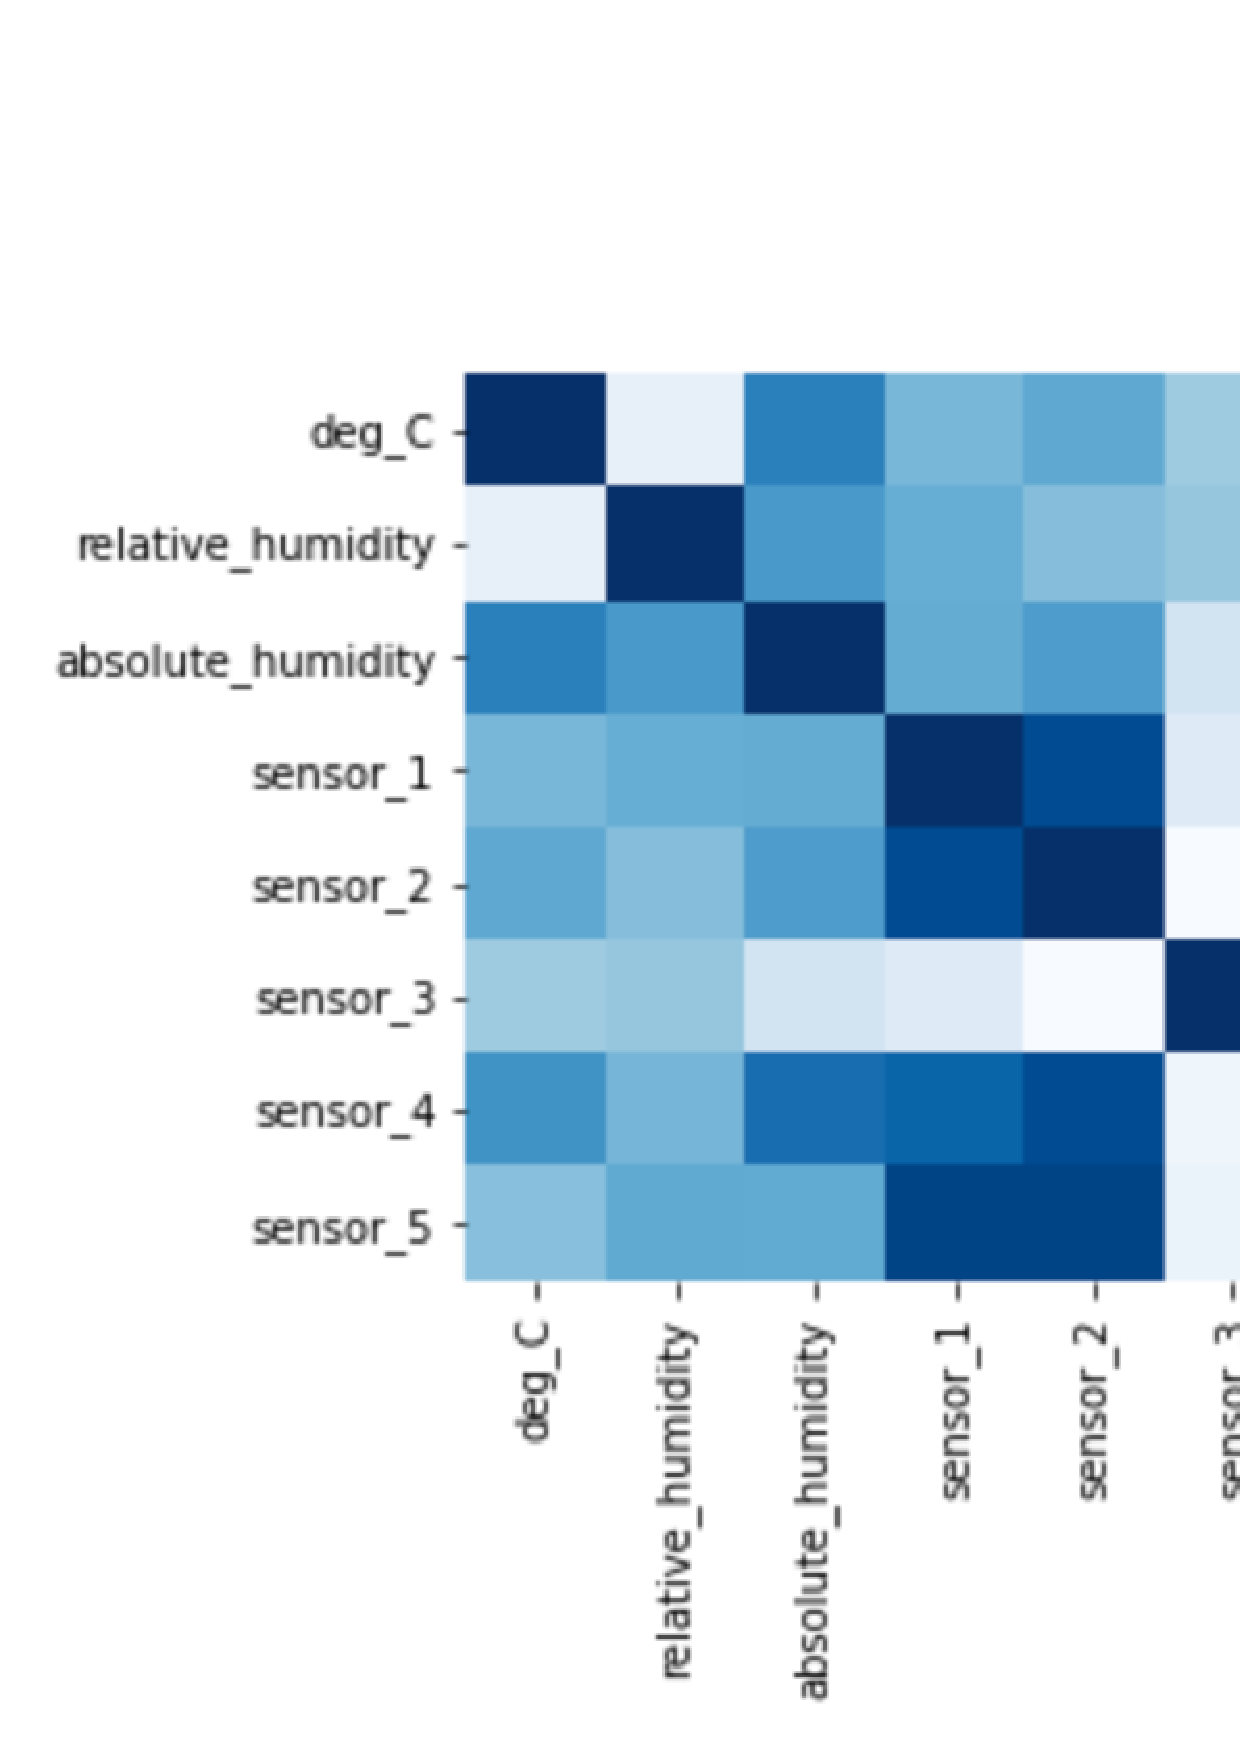
\includegraphics[scale=.8]{templatex/graphics/modelimage/Fig_heatmap.png}

    \end{tikzfigure}%

\hfill

\begin{description}
  	\item[Multicollinearity]
  .Multicollinearity is a aspect which occurs when two or more predictor variables are correlated. As a consequent,
coefficients error may increase. Then the each variables
behave insignificantly, though they should be significant.
\end{description}


\begin{description}
\item[Rigid Regression]
   This is a technique used to implement multicollinearity
of predictor variables which are highly correlated each other
[5]. Generally, rigid regression is same like linear regression
unless it add penalty values to reduce the loss or error of
linear regression. This error can be happen due to bias and/or
variance of the variables
\end{description}
}
%%%%%%%%%% -------------------------------------------------------------------- %%%%%%%%%%


% SECOND column
\column{0.5}
 %Second column with first block's top edge aligned with with previous column's top.

%%%%%%%%%% -------------------------------------------------------------------- %%%%%%%%%%
\block{Preliminaries}{
\begin{description}
    \item
 Making prediction cannot be always
trustworthy to have 100% accuracy.
\end{description}

\begin{tikzfigure}%[Overall architecture of \emph{GOAM} algorithm]
    \includegraphics[scale=.7]{templatex/graphics/modelimage/Bias and Variance.png}
\end{tikzfigure}

\begin{description}
  	\item[Bias Variance and determination of coefficient]
Bias and Variance are prediction errors. These errors are called Bias and Variance.
We use this bias and variance values in the models to state
accuracy levels of proposed models in our evaluation process.
Bias is a training data error while variance is the testing data
error.

\end{description}
}
%%%%%%%%%% -------------------------------------------------------------------- %%%%%%%%%%
% Second column - first block


%%%%%%%%%% -------------------------------------------------------------------- %%%%%%%%%%
\block[titleleft]{Experiment and Evaluations}
{

\begin{description}
  	\item The test data
histogram is properly fitted with train data histogram. Further, in above
However, we use coefficient determination factor to show how
well our proposed models fits the observed data.
\end{description}
\centering
\begin{tabular}{ |c | c | c | c |}
    \toprule
    Method     &  CM  & Benzene& NO     \\
    \midrule
    Bias & 0.38 & 3.379 & 12916.6 \\
    Variance & 0.001 & 0.009 & 30.591 \\
    CD Training & 0.82 & 0.95 & 0.68 \\
    CD Testing & 0.83 & 0.94 & 0.66 \\
     \bottomrule
\end{tabular}

\vspace{.2cm}
\begin{description}
    \item

\end{description}

\begin{description}
\item

\end{description}
\vspace{.5cm}
           
\begin{minipage}{0.3\linewidth}
   \centering
   \begin{tikzfigure}
    \includegraphics[scale=.4]{templatex/graphics/modelimage/Fig_BenzeneModelBehavior.png}
        {\small{Benzene Prediction}}
    \end{tikzfigure}%

\end{minipage}
\hfill
\begin{minipage}{0.3\linewidth}
 \centering
   \begin{tikzfigure}
    \includegraphics[scale=.4]{templatex/graphics/modelimage/Fig_NOxModelBehavior.png}
      {\small{Nitrous oxide Prediction}}
    \end{tikzfigure}%

\end{minipage}
\hfill
\begin{minipage}{0.3\linewidth}
    \centering
    \begin{tikzfigure}
    \includegraphics[scale=.4]{templatex/graphics/modelimage/Fig_CM_ModelAccuracy.png}

   {\small{Carbon monoxide Prediction}}
    \end{tikzfigure}%
 \vspace{.2cm}
\end{minipage}
\begin{description}
  All three models have overall best performance
efficiency. For example, carbon monoxide prediction model
hold 0.82 (82\%) coefficient determination, which indicates
high efficiency of the model. And such, benzene model holds�
0.95 (95\%) coefficient determination, which indicates highest
efficiency. Moreover, compare to the other two models, the
model for nitrous oxide has less efficiency since it has 0.6
coefficient determination.
\end{description}
}
%%%%%%%%%% -------------------------------------------------------------------- %%%%%%%%%%


% Second column - second block
%%%%%%%%%% -------------------------------------------------------------------- %%%%%%%%%%
\block[titlewidthscale=1, bodywidthscale=1]
{Conclusion}
{
\begin{description}
  \item[Problem Definition]
we propose prediction model to predict air
pollution components which are specified as carbon monoxide,
benzene and nitrous oxide. 

  \item[Algorithm]
  Consequently, we use \emph{rigid linear
regression} instead general \emph{linear regression} method. 

  \item[Strategies]
  We uses multiple predictors
such as temperature, absolute and relative humidity and five
sensor data. We identify that these predictors are correlated
among each other. Therefore, we reveals the need of handling
multicollinearity.  We clearly
show the performance efficiency of proposed models using
determination of coefficient, bias and variance scores for each
models.
\item[Recommendations]
Evaluate how
well these prediction models behave on adding more noisy data.
How to affect prediction accuracy by noisy data.
Increase the amount of
predictors to predict air pollution.
\end{description}
}
%%%%%%%%%% -------------------------------------------------------------------- %%%%%%%%%%


% Bottomblock
%%%%%%%%%% -------------------------------------------------------------------- %%%%%%%%%%
\colorlet{notebgcolor}{blue!20}
\colorlet{notefrcolor}{blue!20}
\note[targetoffsetx=8cm, targetoffsety=-4cm, angle=30, rotate=15,
radius=2cm, width=.26\textwidth]{
Acknowledgement
\begin{itemize}
    \item
Kaggle Project and FLIP00 team
 \end{itemize}
}

%\note[targetoffsetx=8cm, targetoffsety=-10cm,rotate=0,angle=180,radius=8cm,width=.46\textwidth,innersep=.1cm]{
%Acknowledgement
%}

%\block[titlewidthscale=0.9, bodywidthscale=0.9]
%{Acknowledgement}{
%}
%%%%%%%%%% -------------------------------------------------------------------- %%%%%%%%%%

\end{columns}


%%%%%%%%%% -------------------------------------------------------------------- %%%%%%%%%%
%[titleleft, titleoffsetx=2em, titleoffsety=1em, bodyoffsetx=2em,%
%roundedcorners=10, linewidth=0mm, titlewidthscale=0.7,%
%bodywidthscale=0.9, titlecenter]

%\colorlet{noteframecolor}{blue!20}
\colorlet{notebgcolor}{blue!20}
\colorlet{notefrcolor}{blue!20}
\note[targetoffsetx=-13cm, targetoffsety=-12cm,rotate=0,angle=180,radius=8cm,width=.96\textwidth,innersep=.4cm]
{
\begin{minipage}{0.3\linewidth}
\centering
\includegraphics[width=24cm]{./graphics/logos/tulip-wordmark.eps}
\end{minipage}
\begin{minipage}{0.7\linewidth}
{ \centering
Kaggle Project and FLIP00 team
}
\end{minipage}
}
%%%%%%%%%% -------------------------------------------------------------------- %%%%%%%%%%


\end{document}

%\endinput
%%
%% End of file `tikzposter-template.tex'.
